\section{Derivation of Fermi energy as function of the Fermi angle}\label{ap:fermi}
Conservation of mass-energy gives:\begin{gather*}
2m_0c^2 = cp_1 + cp_2,
\end{gather*}where $p_1$ and $p_2$ are the length of the corresponding momentum-vectors. If $\boldsymbol{p_e}$ has length $p_e$, an arbitrary angle $\varphi$ with the $x$-axis and setting the momentum $\boldsymbol{p_1}$ of one of the photons in the $x$-direction the following situation occurs:
\begin{figure}[H]
	\centering
	\begin{subfigure}[t]{0.45\linewidth}
		\centering
		\resizebox{\linewidth}{!}{\begin{tikzpicture}[
	level/.style={black,thick},
    sublevel/.style={black,densely dashed},
    momentum/.style={black,->,>=stealth'}]
    
    % Coordinate system
    \draw (-1.5,0) -- (1.5,0) node[right] {$x$};
    \draw (0,-1.5) -- (0,1.5) node[above] {$y$};
    
    % define coordinates
    \coordinate (O) at (0,0) ;
    \coordinate (A) at (1,1) ;
    
    % Momentum vector
	\draw[momentum] (O) -- (A);
    
    % Angle arc
    \draw (6mm,0) arc [start angle=0, end angle=45, radius=6mm] node[xshift=0.3cm, yshift=-0.13cm] {$\varphi$};
    
    % Dotted lines
    \draw[dashed]  (1,0) node[below] {$p_{e_{x}}$} -- (1,1) 
    (0,1) node[left] {$p_{e_{y}}$} -- (1,1) node[above right] {$\boldsymbol{p_e}$};

  \end{tikzpicture}}
		\caption{Momentum of an electron $\boldsymbol{p_e}$ with an angle $\varphi$ to the $x$-axis}
		\label{fig:momentumvectors1}
	\end{subfigure}
	~
	\begin{subfigure}[t]{0.45\linewidth}
		\centering
		\resizebox{\linewidth}{!}{\begin{tikzpicture}[
	level/.style={black,thick},
    sublevel/.style={black,densely dashed},
    momentum/.style={black,->,>=stealth'}]
    
    % Coordinate system
    \draw (-1.5,0) -- (1.5,0) node[right] {$x$};
    \draw (0,-1.5) -- (0,1.5) node[above] {$y$};
    
    % define coordinates
    \coordinate (O) at (0,0);
    \coordinate (A) at (-1,1);
    \coordinate (B) at (1,0);
    
    % Momentum vectors
	\draw[momentum] (O) -- (A) node[above left] {$\boldsymbol{p_2}$};
	\draw[momentum] (O) -- (B) node[below] {$\boldsymbol{p_1}$};
    
    % Angle arc
    \draw (-6mm,0) arc [start angle=0, end angle=-45, radius=-6mm] node[xshift=-0.3cm, yshift=-0.13cm] {$\theta$};
    
  \end{tikzpicture}}
		\caption{Momentum of the two photons $\boldsymbol{p_1}$ and $\boldsymbol{p_2}$, with the direction of $\boldsymbol{p_1}$ fixed to the $x$-axis and $\boldsymbol{p_2}$ has an angle $\theta$ with the negative $x$-axis.}
		\label{fig:momentumvectors2}
	\end{subfigure}
	\caption{Schematic of the momentum-vectors of the electron and two photons, assuming the positron has no momentum during the annihilation process.}
	\label{fig:momentumvectoren}
\end{figure}Conservation of linear momentum implies the conservation of both the $x$- and $y$-component of the momentum, which gives the following equations:
\begin{align*}
p_e\cos(\varphi) &= p_1 - p_2\cos(\theta)\\
p_e\sin(\varphi) &= p_2\sin(\theta).
\end{align*} From which it follows that:
\begin{align*}
p_2 &= p_e \frac{\sin(\varphi)}{\sin(\theta)}\\
p_1 &= p_e\cos(\theta) + p_2 \cos(\theta)\\
&= p_e \cos(\theta) + p_e \cos(\theta) \frac{\sin(\varphi)}{\sin(\theta)}\\
2m_0c^2 &= cp_1 + p_2\\
&= cp_e\left(\cos(\theta) + \cos(\theta) \frac{\sin(\varphi)}{\sin(\theta)}+\frac{\sin(\varphi)}{\sin(\theta)}\right).
\end{align*} For low energies of the electron $p_e \ll m_0c$, and from that it follows that $\theta$ is small which implies that the small-angle approximation can be used (i.e. $\sin(\theta)\approx \theta$ and $\cos(\theta) \approx 1$): \begin{align*}
2m_0c^2 &= cp_e\left(\cos(\theta) + \cos(\theta;) \frac{\sin(\varphi)}{\sin(\theta)}+\frac{\sin(\varphi)}{\sin(\theta)}\right)\\
2m_0c &\approx p_e\left(1 + 2\frac{\sin(\varphi)}\theta \right)\\
&\approx p_e +\frac{2p_e\sin(\varphi)}{\theta}\\
2m_0c - p_e &= \frac{2p_e\sin(\varphi)}{\theta}\\
\theta &= \frac{2p_e\sin(\varphi)}{2m_0c-p_e}\\
\theta &\approx \frac{p_y}{m_0c}.
\end{align*}

\section{Measuring the relation between channels and energy}\label{ap:na22}
$^{22}$Na decays into $^{22}$Ne by different means. Most prominently (90\% of the time) it will decay to the 1274~keV energy level of $^{22}$Ne, emitting a 545~keV positron in the process. 10\% of the time an electron will be absorbed instead of a positron being emitted. The $^{22}$Ne will fall to the ground state within picoseconds by emitting 1274~keV $\gamma$-radiation. On rare occasions, 0.05\% of the time, the $^{22}$Na decays directly into the $^{22}$Ne ground state by emitting a 1.83~MeV positron (Figure \ref{fig:22na-decay}) \cite{RadiationEnergies}. A measurement of a $^{22}$Na source with aluminium around it (see figure \ref{fig:bg22na}) shows these transitions, where the peak between 500~keV and 600~keV is from annihilation events, not from the 454~keV positrons. 
\begin{figure}[H]
\centering
\resizebox{\columnwidth}{!}{ \begin{tikzpicture}[
    level/.style={black,thick},
    sublevel/.style={black,densely dashed},
    transition/.style={black,->,>=stealth',shorten >=1pt},
    ionization/.style={transition,dashed},
    radiative/.style={transition,decorate,decoration={snake,amplitude=1.5}},
    indirectradiative/.style={radiative,densely dashed},
    nonradiative/.style={transition,dashed},
  ]
  \coordinate (sublevel) at (0, 8pt);

  % Ne levels
  \coordinate (S00) at (0, 0);
  \coordinate (S22) at (0, 3);

  % Draw main levels
  \draw[level] (S22) node[left] {\footnotesize $^{22}$Ne} -- +(3, 0) node[above left=-.05cm] {\tiny 1274~keV};
  \draw[level] (S00) node[left] {\footnotesize $^{22}$Ne} -- +(3, 0) node[above left=-.05cm] {\tiny 0~keV};

  % NA levels
  \coordinate (T22) at (3.5,4.5);
      
  % Draw main levels
  \foreach \level/\text in {22/2}
    \draw[level] (T\level) node[left] {\footnotesize $^{\level}$Na} -- +(3,0);

  % Transition arrows
  \draw[ionization,name path=crossing] ($(T22) + (1.5,0) - (0,0.1)$) --
    ($(S22) + (1.5,0.1)$);
  \node[right,align=center] at ($(T22) + (.3,-.75)$)
    {\footnotesize $\beta^{+}$};
    
    
  \draw[ionization,name path=crossing] ($(T22) + (1.5,0) - (0,0.1)$) --
    ($(S00) + (1.5,0.1)$);
  \node[right,align=center] at ($(T22) + (0,-2.25)$)
    {\footnotesize $\beta^{+}$};
    
  \draw[radiative,name path=crossing] ($(S22) + (1.5,0) - (0,0.1)$) --
    ($(S00) + (1.5,0.1)$);
  \node[right,align=center] at (1.75,1.5)
    {\footnotesize $\gamma$};
    
    
  \end{tikzpicture}}
\caption{Decay scheme of $^{22}$Na source. A large portion (90~\%) will disintegrate to the 1.275~MeV level of $^{22}$Ne (545~keV $\beta^{+}$), which can fall to the ground state (1.275~MeV $\gamma$). A small fraction (0.05~\%) will decay directly to the $^{22}$Ne ground state (1.83~MeV $\beta^{+}$).}
\label{fig:22na-decay}
\end{figure}
The standard peak detection algorithm in MATLAB is used to find the peaks in the energy spectrum. The algorithm found two peaks at channels 1001 and 2499, corresponding to 511~keV and 1.275~MeV respectively. From this it follows that the channels and energies differ a factor 0.5105.
	
\section{Unfiltered energy spectrum}\label{ap:bg22na}
\begin{figure}[H]
\centering
\resizebox{\columnwidth}{!}{% GNUPLOT: LaTeX picture with Postscript
\begingroup
  \makeatletter
  \providecommand\color[2][]{%
    \GenericError{(gnuplot) \space\space\space\@spaces}{%
      Package color not loaded in conjunction with
      terminal option `colourtext'%
    }{See the gnuplot documentation for explanation.%
    }{Either use 'blacktext' in gnuplot or load the package
      color.sty in LaTeX.}%
    \renewcommand\color[2][]{}%
  }%
  \providecommand\includegraphics[2][]{%
    \GenericError{(gnuplot) \space\space\space\@spaces}{%
      Package graphicx or graphics not loaded%
    }{See the gnuplot documentation for explanation.%
    }{The gnuplot epslatex terminal needs graphicx.sty or graphics.sty.}%
    \renewcommand\includegraphics[2][]{}%
  }%
  \providecommand\rotatebox[2]{#2}%
  \@ifundefined{ifGPcolor}{%
    \newif\ifGPcolor
    \GPcolortrue
  }{}%
  \@ifundefined{ifGPblacktext}{%
    \newif\ifGPblacktext
    \GPblacktextfalse
  }{}%
  % define a \g@addto@macro without @ in the name:
  \let\gplgaddtomacro\g@addto@macro
  % define empty templates for all commands taking text:
  \gdef\gplbacktext{}%
  \gdef\gplfronttext{}%
  \makeatother
  \ifGPblacktext
    % no textcolor at all
    \def\colorrgb#1{}%
    \def\colorgray#1{}%
  \else
    % gray or color?
    \ifGPcolor
      \def\colorrgb#1{\color[rgb]{#1}}%
      \def\colorgray#1{\color[gray]{#1}}%
      \expandafter\def\csname LTw\endcsname{\color{white}}%
      \expandafter\def\csname LTb\endcsname{\color{black}}%
      \expandafter\def\csname LTa\endcsname{\color{black}}%
      \expandafter\def\csname LT0\endcsname{\color[rgb]{1,0,0}}%
      \expandafter\def\csname LT1\endcsname{\color[rgb]{0,1,0}}%
      \expandafter\def\csname LT2\endcsname{\color[rgb]{0,0,1}}%
      \expandafter\def\csname LT3\endcsname{\color[rgb]{1,0,1}}%
      \expandafter\def\csname LT4\endcsname{\color[rgb]{0,1,1}}%
      \expandafter\def\csname LT5\endcsname{\color[rgb]{1,1,0}}%
      \expandafter\def\csname LT6\endcsname{\color[rgb]{0,0,0}}%
      \expandafter\def\csname LT7\endcsname{\color[rgb]{1,0.3,0}}%
      \expandafter\def\csname LT8\endcsname{\color[rgb]{0.5,0.5,0.5}}%
    \else
      % gray
      \def\colorrgb#1{\color{black}}%
      \def\colorgray#1{\color[gray]{#1}}%
      \expandafter\def\csname LTw\endcsname{\color{white}}%
      \expandafter\def\csname LTb\endcsname{\color{black}}%
      \expandafter\def\csname LTa\endcsname{\color{black}}%
      \expandafter\def\csname LT0\endcsname{\color{black}}%
      \expandafter\def\csname LT1\endcsname{\color{black}}%
      \expandafter\def\csname LT2\endcsname{\color{black}}%
      \expandafter\def\csname LT3\endcsname{\color{black}}%
      \expandafter\def\csname LT4\endcsname{\color{black}}%
      \expandafter\def\csname LT5\endcsname{\color{black}}%
      \expandafter\def\csname LT6\endcsname{\color{black}}%
      \expandafter\def\csname LT7\endcsname{\color{black}}%
      \expandafter\def\csname LT8\endcsname{\color{black}}%
    \fi
  \fi
  \setlength{\unitlength}{0.0500bp}%
  \begin{picture}(5668.00,3400.00)%
    \gplgaddtomacro\gplbacktext{%
      \csname LTb\endcsname%
      \put(980,640){\makebox(0,0)[r]{\strut{} 0}}%
      \csname LTb\endcsname%
      \put(980,920){\makebox(0,0)[r]{\strut{} 200}}%
      \csname LTb\endcsname%
      \put(980,1200){\makebox(0,0)[r]{\strut{} 400}}%
      \csname LTb\endcsname%
      \put(980,1480){\makebox(0,0)[r]{\strut{} 600}}%
      \csname LTb\endcsname%
      \put(980,1760){\makebox(0,0)[r]{\strut{} 800}}%
      \csname LTb\endcsname%
      \put(980,2039){\makebox(0,0)[r]{\strut{} 1000}}%
      \csname LTb\endcsname%
      \put(980,2319){\makebox(0,0)[r]{\strut{} 1200}}%
      \csname LTb\endcsname%
      \put(980,2599){\makebox(0,0)[r]{\strut{} 1400}}%
      \csname LTb\endcsname%
      \put(980,2879){\makebox(0,0)[r]{\strut{} 1600}}%
      \csname LTb\endcsname%
      \put(980,3159){\makebox(0,0)[r]{\strut{} 1800}}%
      \csname LTb\endcsname%
      \put(1100,440){\makebox(0,0){\strut{} 0}}%
      \csname LTb\endcsname%
      \put(1941,440){\makebox(0,0){\strut{} 500}}%
      \csname LTb\endcsname%
      \put(2783,440){\makebox(0,0){\strut{} 1000}}%
      \csname LTb\endcsname%
      \put(3624,440){\makebox(0,0){\strut{} 1500}}%
      \csname LTb\endcsname%
      \put(4466,440){\makebox(0,0){\strut{} 2000}}%
      \csname LTb\endcsname%
      \put(5307,440){\makebox(0,0){\strut{} 2500}}%
      \put(160,1899){\rotatebox{-270}{\makebox(0,0){\strut{}Counts}}}%
      \put(3203,140){\makebox(0,0){\strut{}Energy [keV]}}%
    }%
    \gplgaddtomacro\gplfronttext{%
    }%
    \gplbacktext
    \put(0,0){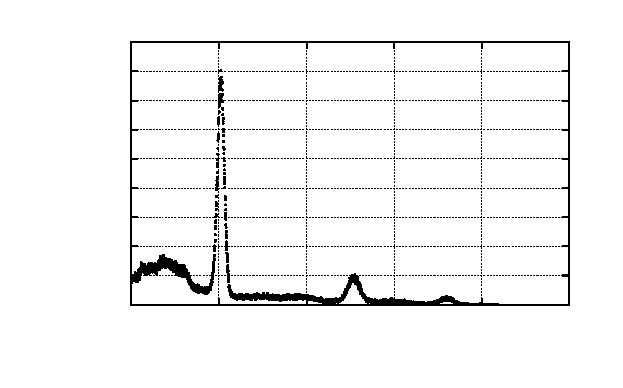
\includegraphics{bg22na}}%
    \gplfronttext
  \end{picture}%
\endgroup
}
\caption{Energy spectrum without acquisition windows on the SCA's. Besides the 511~keV annihilation photons, radiation from Compton scattering and the $^{22}$Na isotope falling to the ground state (1274.5~keV) is present. The small peak around 1.8~MeV is due to 511 and 1274.5~keV photons being registered as one particle by the detector.}
\label{fig:bg22na}
\end{figure}

\section{Energy spectrum filtered for 511~keV photons}\label{ap:bg_511}
\begin{figure}[H]
\centering
\resizebox{\columnwidth}{!}{% GNUPLOT: LaTeX picture with Postscript
\begingroup
  \makeatletter
  \providecommand\color[2][]{%
    \GenericError{(gnuplot) \space\space\space\@spaces}{%
      Package color not loaded in conjunction with
      terminal option `colourtext'%
    }{See the gnuplot documentation for explanation.%
    }{Either use 'blacktext' in gnuplot or load the package
      color.sty in LaTeX.}%
    \renewcommand\color[2][]{}%
  }%
  \providecommand\includegraphics[2][]{%
    \GenericError{(gnuplot) \space\space\space\@spaces}{%
      Package graphicx or graphics not loaded%
    }{See the gnuplot documentation for explanation.%
    }{The gnuplot epslatex terminal needs graphicx.sty or graphics.sty.}%
    \renewcommand\includegraphics[2][]{}%
  }%
  \providecommand\rotatebox[2]{#2}%
  \@ifundefined{ifGPcolor}{%
    \newif\ifGPcolor
    \GPcolortrue
  }{}%
  \@ifundefined{ifGPblacktext}{%
    \newif\ifGPblacktext
    \GPblacktextfalse
  }{}%
  % define a \g@addto@macro without @ in the name:
  \let\gplgaddtomacro\g@addto@macro
  % define empty templates for all commands taking text:
  \gdef\gplbacktext{}%
  \gdef\gplfronttext{}%
  \makeatother
  \ifGPblacktext
    % no textcolor at all
    \def\colorrgb#1{}%
    \def\colorgray#1{}%
  \else
    % gray or color?
    \ifGPcolor
      \def\colorrgb#1{\color[rgb]{#1}}%
      \def\colorgray#1{\color[gray]{#1}}%
      \expandafter\def\csname LTw\endcsname{\color{white}}%
      \expandafter\def\csname LTb\endcsname{\color{black}}%
      \expandafter\def\csname LTa\endcsname{\color{black}}%
      \expandafter\def\csname LT0\endcsname{\color[rgb]{1,0,0}}%
      \expandafter\def\csname LT1\endcsname{\color[rgb]{0,1,0}}%
      \expandafter\def\csname LT2\endcsname{\color[rgb]{0,0,1}}%
      \expandafter\def\csname LT3\endcsname{\color[rgb]{1,0,1}}%
      \expandafter\def\csname LT4\endcsname{\color[rgb]{0,1,1}}%
      \expandafter\def\csname LT5\endcsname{\color[rgb]{1,1,0}}%
      \expandafter\def\csname LT6\endcsname{\color[rgb]{0,0,0}}%
      \expandafter\def\csname LT7\endcsname{\color[rgb]{1,0.3,0}}%
      \expandafter\def\csname LT8\endcsname{\color[rgb]{0.5,0.5,0.5}}%
    \else
      % gray
      \def\colorrgb#1{\color{black}}%
      \def\colorgray#1{\color[gray]{#1}}%
      \expandafter\def\csname LTw\endcsname{\color{white}}%
      \expandafter\def\csname LTb\endcsname{\color{black}}%
      \expandafter\def\csname LTa\endcsname{\color{black}}%
      \expandafter\def\csname LT0\endcsname{\color{black}}%
      \expandafter\def\csname LT1\endcsname{\color{black}}%
      \expandafter\def\csname LT2\endcsname{\color{black}}%
      \expandafter\def\csname LT3\endcsname{\color{black}}%
      \expandafter\def\csname LT4\endcsname{\color{black}}%
      \expandafter\def\csname LT5\endcsname{\color{black}}%
      \expandafter\def\csname LT6\endcsname{\color{black}}%
      \expandafter\def\csname LT7\endcsname{\color{black}}%
      \expandafter\def\csname LT8\endcsname{\color{black}}%
    \fi
  \fi
  \setlength{\unitlength}{0.0500bp}%
  \begin{picture}(5668.00,3400.00)%
    \gplgaddtomacro\gplbacktext{%
      \csname LTb\endcsname%
      \put(980,640){\makebox(0,0)[r]{\strut{} 0}}%
      \csname LTb\endcsname%
      \put(980,920){\makebox(0,0)[r]{\strut{} 200}}%
      \csname LTb\endcsname%
      \put(980,1200){\makebox(0,0)[r]{\strut{} 400}}%
      \csname LTb\endcsname%
      \put(980,1480){\makebox(0,0)[r]{\strut{} 600}}%
      \csname LTb\endcsname%
      \put(980,1760){\makebox(0,0)[r]{\strut{} 800}}%
      \csname LTb\endcsname%
      \put(980,2039){\makebox(0,0)[r]{\strut{} 1000}}%
      \csname LTb\endcsname%
      \put(980,2319){\makebox(0,0)[r]{\strut{} 1200}}%
      \csname LTb\endcsname%
      \put(980,2599){\makebox(0,0)[r]{\strut{} 1400}}%
      \csname LTb\endcsname%
      \put(980,2879){\makebox(0,0)[r]{\strut{} 1600}}%
      \csname LTb\endcsname%
      \put(980,3159){\makebox(0,0)[r]{\strut{} 1800}}%
      \csname LTb\endcsname%
      \put(1100,440){\makebox(0,0){\strut{} 0}}%
      \csname LTb\endcsname%
      \put(1941,440){\makebox(0,0){\strut{} 500}}%
      \csname LTb\endcsname%
      \put(2783,440){\makebox(0,0){\strut{} 1000}}%
      \csname LTb\endcsname%
      \put(3624,440){\makebox(0,0){\strut{} 1500}}%
      \csname LTb\endcsname%
      \put(4466,440){\makebox(0,0){\strut{} 2000}}%
      \csname LTb\endcsname%
      \put(5307,440){\makebox(0,0){\strut{} 2500}}%
      \put(160,1899){\rotatebox{-270}{\makebox(0,0){\strut{}Counts}}}%
      \put(3203,140){\makebox(0,0){\strut{}Energy [keV]}}%
    }%
    \gplgaddtomacro\gplfronttext{%
    }%
    \gplbacktext
    \put(0,0){\includegraphics{bg_511}}%
    \gplfronttext
  \end{picture}%
\endgroup
}
\caption{Energy spectrum after calibrating the acquisition windows on the SCA's, so that only 511~keV radiation is registered.}
\label{fig:bg_511}
\end{figure}

\section{Radiation risk analysis}
The equivalent dose $H_T$ is found by multiplying the dose averaged over the tissue $D$ with a weighting factor $w_R$:
\begin{equation}
H_T = w_R \cdot D.
\label{eq:equiv}
\end{equation}The dose is measured in gray (Gy or J$\cdot$kg$^{-1}$), for this analysis a weighting factor of 1 used, this corresponds to a full body exposure.

The dose can be found with the following equation:
\begin{equation}
D = \frac{\Gamma A}{r^2} e^{-\mu d}
\label{eq:avg}
\end{equation} where $\Gamma$ stands for the source constant in Gy$\cdot$m$^2$$\cdot$Bq$^{-1}\cdot$h$^{-1}$, $A$ for the activity in Bq and $r$ is the distance from the observer to the source in meters. $\mu$ is the total linear interaction coefficient. It is an inherent property of the shielding material and the value is obtained from literature. $d$ is the thickness of the shielding material. 

In the setup a $^{22}$Na isotope is used as source. The activity was measured on July \nth{1} 2006 to be 4~MBq. $^{22}$Na has a half-life of 2.6 years, giving a current activity of \begin{gather*}
	A = A_0e^{-\frac{t\ln(2)}{\tau}} = 4\cdot e^{-\frac{7.6\ln(2)}{2.6}} \approx 0.5~\text{MBq}.
\end{gather*}

When charged particles particles are slowed down by other charged particles the kinetic energy is converted to a photon. This process is called Bremsstrahlung, and occurs in the experiment when the $\beta^+$-particles are slowed by the electrons in the atomic nuclei of the aluminium. The fraction $g$ of the energy that is converted in such a case is given by\begin{equation}
g = 2 \cdot 10^{-4} \cdot Z \cdot E_{\beta, max},
\label{eq:g}
\end{equation}with $E_{\beta, max}$ the maximum energy of the $\beta$-particles (in MeV) and $Z$ the atomic number of the material where the slowing down occurs. 

\subsection*{Expected dose}
Risk of exposure comes from 1.83~MeV, 545~keV $\beta^{+}$ particles and 1.275~MeV $\gamma$-radation. To determine the risk of exposure from $\beta$-radiation, the range of the $\beta$ particles in aluminium is determined with: \begin{equation*}
R_{\beta,\text{lin.}}=\frac{0.5 E_{\beta,\text{max}}}{\rho},
\end{equation*} with $R_{\beta,\text{lin.}}$ in cm, $E$ in MeV and $\uprho$ is density of the surrounding material in g$\cdot$cm$^{3}$. Aluminium has a density of 2.70~g$\cdot$cm$^{3}$ and $E_{\beta,\text{max}}$~=~1.83~MeV, this gives a range R$_{\beta,\text{lin.}}$~=~0.34~cm. The aluminium surrounding the $^{22}$Na is has a thickness of 4~mm, thus there is no risk of direct exposure from $\beta$-radiation.

Another risk is Bremsstrahlung. For the experiment, $Z$ = 13 and $E_{\beta, max}$ = 1.83~MeV, it then follows equation \ref{eq:g} that $g\approx 0.005$. The converted energy is then equal to $0.005\cdot 1.83~\text{MeV}\approx8.7~\text{keV}$. Approximately 0.06\% of the activity belongs to $\beta^+$ decay with an energy of 1.83~MeV, meaning that on average the Bremsstrahlung is $8.7\cdot 0.5\cdot 0.0006 \approx 2.6~\text{eV}\cdot \text{s}^{-1}$, which is negligible and poses no risk.

Tabel \ref{tab:na-prop} and \ref{tab:setup} show some relevant values for the source.
\begin{table}[H]
		\caption{$^{22}$Na source properties}
    \begin{tabularx}{\linewidth}{l X}
			Property & Value \\ \hline\hline
      $\Gamma$ & $3.3\cdot 10^{-13}$~Gy$\cdot$m$^2$$\cdot$Bq$^{-1}\cdot$h$^{-1}$ \\
      $A$ & 0.5 MBq \\ \hline
    \end{tabularx}
    \label{tab:na-prop}
\end{table}

\begin{table}[H]
    \caption{Setup properties}
		\begin{tabularx}{\linewidth}{l X}
			Property & Value \\ \hline\hline
      $\mu$ & 0.6452 cm$^{-1}$ \\
      $d$ & 0.05~m \\
      $r$ & 0.5~m \\\hline
    \end{tabularx}
    \label{tab:setup}
\end{table}Filling these values in equations \ref{eq:equiv} and \ref{eq:avg} gives the equivalent dose: $H_T~\approx~6.4\cdot 10^{-1}$ pSv$\cdot$h$^{-1}$. There will be two measurements, each with an attendance duration of 3~hours. Thus the total equivalent dose will be $6~H_T = 3.8$~pSv. This is well below the maximum allowed dose for a student (6~mSv/year), or the effective dose for Dutch citizens (2.4 mSv/year)  \cite{Brouwer}.

